\documentclass[14pt]{extbook}
\usepackage{multicol, enumerate, enumitem, hyperref, color, soul, setspace, parskip, fancyhdr} %General Packages
\usepackage{amssymb, amsthm, amsmath, latexsym, units, mathtools} %Math Packages
\everymath{\displaystyle} %All math in Display Style
% Packages with additional options
\usepackage[headsep=0.5cm,headheight=12pt, left=1 in,right= 1 in,top= 1 in,bottom= 1 in]{geometry}
\usepackage[usenames,dvipsnames]{xcolor}
\usepackage{dashrule}  % Package to use the command below to create lines between items
\newcommand{\litem}[1]{\item#1\hspace*{-1cm}\rule{\textwidth}{0.4pt}}
\pagestyle{fancy}
\lhead{Progress Quiz 7}
\chead{}
\rhead{Version B}
\lfoot{4173-5738}
\cfoot{}
\rfoot{Spring 2021}
\begin{document}

\begin{enumerate}
\litem{
First, find the equation of the line containing the two points below. Then, write the equation as $ y=mx+b $ and choose the intervals that contain $m$ and $b$.\[ (-11, -5) \text{ and } (2, 11) \]\begin{enumerate}[label=\Alph*.]
\item \( m \in [-1.4, -0.1] \hspace*{3mm} b \in [13.1, 15.9] \)
\item \( m \in [0.8, 2.7] \hspace*{3mm} b \in [-10, -6.3] \)
\item \( m \in [0.8, 2.7] \hspace*{3mm} b \in [5.4, 7.6] \)
\item \( m \in [0.8, 2.7] \hspace*{3mm} b \in [8.1, 8.9] \)
\item \( m \in [0.8, 2.7] \hspace*{3mm} b \in [8.7, 10.5] \)

\end{enumerate} }
\litem{
Write the equation of the line in the graph below in Standard form $Ax+By=C$. Then, choose the intervals that contain $A, B, \text{ and } C$.
\begin{center}
    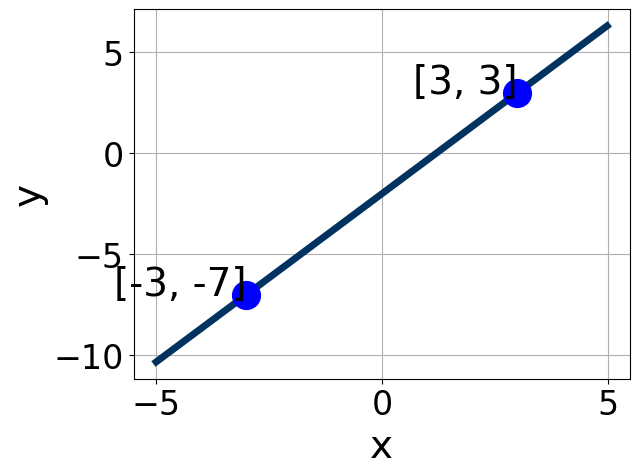
\includegraphics[width=0.5\textwidth]{../Figures/linearGraphToStandardB.png}
\end{center}
\begin{enumerate}[label=\Alph*.]
\item \( A \in [-4.67, 0.33], \hspace{3mm} B \in [0.59, 1.78], \text{ and } \hspace{3mm} C \in [-2, -1] \)
\item \( A \in [3, 7], \hspace{3mm} B \in [-4, -2.48], \text{ and } \hspace{3mm} C \in [4, 9] \)
\item \( A \in [-4.67, 0.33], \hspace{3mm} B \in [-1.21, -0.03], \text{ and } \hspace{3mm} C \in [0, 4] \)
\item \( A \in [3, 7], \hspace{3mm} B \in [2.04, 4.04], \text{ and } \hspace{3mm} C \in [-8, -5] \)
\item \( A \in [-6, -3], \hspace{3mm} B \in [2.04, 4.04], \text{ and } \hspace{3mm} C \in [-8, -5] \)

\end{enumerate} }
\litem{
Solve the equation below. Then, choose the interval that contains the solution.\[ -4(-2x -17) = -10(9x + 3) \]\begin{enumerate}[label=\Alph*.]
\item \( x \in [0.34, 0.4] \)
\item \( x \in [0.41, 0.53] \)
\item \( x \in [-0.42, -0.34] \)
\item \( x \in [-1.07, -0.97] \)
\item \( \text{There are no real solutions.} \)

\end{enumerate} }
\litem{
Solve the equation below. Then, choose the interval that contains the solution.\[ -17(-8x -10) = -13(-3x -11) \]\begin{enumerate}[label=\Alph*.]
\item \( x \in [3, 3.3] \)
\item \( x \in [-1.6, 0.1] \)
\item \( x \in [-2.3, -1.2] \)
\item \( x \in [-3.3, -3] \)
\item \( \text{There are no real solutions.} \)

\end{enumerate} }
\litem{
Find the equation of the line described below. Write the linear equation as $ y=mx+b $ and choose the intervals that contain $m$ and $b$.\[ \text{Parallel to } 7 x + 8 y = 8 \text{ and passing through the point } (-7, -9). \]\begin{enumerate}[label=\Alph*.]
\item \( m \in [-1.51, -0.99] \hspace*{3mm} b \in [-15.29, -13.93] \)
\item \( m \in [-0.99, -0.17] \hspace*{3mm} b \in [-15.29, -13.93] \)
\item \( m \in [-0.99, -0.17] \hspace*{3mm} b \in [-2.16, -1.42] \)
\item \( m \in [-0.99, -0.17] \hspace*{3mm} b \in [14.33, 16.04] \)
\item \( m \in [0.55, 1.34] \hspace*{3mm} b \in [-3.64, -2.72] \)

\end{enumerate} }
\litem{
First, find the equation of the line containing the two points below. Then, write the equation as $ y=mx+b $ and choose the intervals that contain $m$ and $b$.\[ (11, 6) \text{ and } (2, -11) \]\begin{enumerate}[label=\Alph*.]
\item \( m \in [-3.7, -1.2] \hspace*{3mm} b \in [-7.6, -6.3] \)
\item \( m \in [1.6, 3.9] \hspace*{3mm} b \in [-14, -8.8] \)
\item \( m \in [1.6, 3.9] \hspace*{3mm} b \in [13.8, 16.5] \)
\item \( m \in [1.6, 3.9] \hspace*{3mm} b \in [-6.7, -4] \)
\item \( m \in [1.6, 3.9] \hspace*{3mm} b \in [-17.2, -14.2] \)

\end{enumerate} }
\litem{
Find the equation of the line described below. Write the linear equation as $ y=mx+b $ and choose the intervals that contain $m$ and $b$.\[ \text{Parallel to } 4 x - 5 y = 6 \text{ and passing through the point } (-4, -6). \]\begin{enumerate}[label=\Alph*.]
\item \( m \in [0.64, 0.94] \hspace*{3mm} b \in [-2.47, -1.18] \)
\item \( m \in [-1.54, -0.1] \hspace*{3mm} b \in [-10.84, -8.06] \)
\item \( m \in [0.93, 1.67] \hspace*{3mm} b \in [-4.01, -2.42] \)
\item \( m \in [0.64, 0.94] \hspace*{3mm} b \in [-4.01, -2.42] \)
\item \( m \in [0.64, 0.94] \hspace*{3mm} b \in [1.3, 4.14] \)

\end{enumerate} }
\litem{
Solve the linear equation below. Then, choose the interval that contains the solution.\[ \frac{5x + 6}{5} - \frac{-6x + 3}{8} = \frac{6x + 8}{3} \]\begin{enumerate}[label=\Alph*.]
\item \( x \in [-5.37, -2.37] \)
\item \( x \in [-0.63, 2.37] \)
\item \( x \in [-23, -18] \)
\item \( x \in [-11.37, -6.37] \)
\item \( \text{There are no real solutions.} \)

\end{enumerate} }
\litem{
Solve the linear equation below. Then, choose the interval that contains the solution.\[ \frac{-8x -9}{7} - \frac{-5x -6}{8} = \frac{3x + 8}{5} \]\begin{enumerate}[label=\Alph*.]
\item \( x \in [-10, -8] \)
\item \( x \in [-2.7, -0.9] \)
\item \( x \in [-0.9, 0] \)
\item \( x \in [-4.5, -2.2] \)
\item \( \text{There are no real solutions.} \)

\end{enumerate} }
\litem{
Write the equation of the line in the graph below in Standard form $Ax+By=C$. Then, choose the intervals that contain $A, B, \text{ and } C$.
\begin{center}
    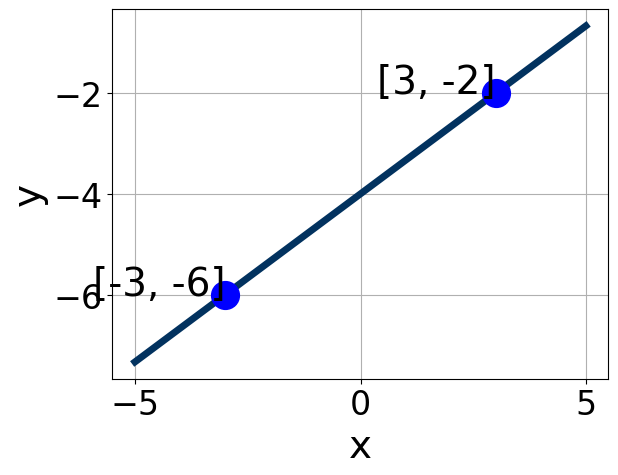
\includegraphics[width=0.5\textwidth]{../Figures/linearGraphToStandardCopyB.png}
\end{center}
\begin{enumerate}[label=\Alph*.]
\item \( A \in [-1.8, -0.3], \hspace{3mm} B \in [-1.31, -0.87], \text{ and } \hspace{3mm} C \in [3, 5] \)
\item \( A \in [0.2, 5.6], \hspace{3mm} B \in [2.7, 4.31], \text{ and } \hspace{3mm} C \in [-22, -9] \)
\item \( A \in [0.2, 5.6], \hspace{3mm} B \in [-3.55, -2.55], \text{ and } \hspace{3mm} C \in [9, 15] \)
\item \( A \in [-3.6, -0.9], \hspace{3mm} B \in [2.7, 4.31], \text{ and } \hspace{3mm} C \in [-22, -9] \)
\item \( A \in [-1.8, -0.3], \hspace{3mm} B \in [0.2, 2.06], \text{ and } \hspace{3mm} C \in [-11, 1] \)

\end{enumerate} }
\end{enumerate}

\end{document}